Dans ce chapitre, nous présentons un tour d'horizon des techniques existantes
permettant d'analyser des programmes. Un accent est mis sur la propriété de
sûreté décrite dans le chapitre~\ref{cha:os}, mais on ne se limite pas à
celle-ci.

L'analyse statique de programmes est un sujet de recherche actif depuis
l'apparition de la science informatique.

\section{Taxonomie}

\paragraph{Techniques statiques et dynamiques :} l'analyse peut être faite au
moment de la compilation, ou au moment de l'exécution. En général on peut
obtenir des informations plus précises de manière dynamique, mais cela ne prend
en compte que les parties du programme qui seront vraiment exécutées. Un autre
problème des techniques dynamiques est qu'il est souvent nécessaire
d'instrumenter l'environnement d'exécution (ce qui --- dans le cas où cela est
possible --- peut se traduire par un impact en performances). L'approche
statique, en revanche, nécessite de construire à l'arrêt une carte mentale du
programme, ce qui n'est pas toujours possible dans certains langages.

Dans la suite, nous considérerons essentiellement des techniques statiques,
précisant le contraire lorsque c'est nécessaire.

\paragraph{Cohérence et complétude :} le but d'une analyse statique est de
catégoriser les programmes selon leurs caractéristiques à l'exécution. Or,

\begin{theorem}[de Rice]
  Toute propriété non triviale sur le comportement dynamique des programmes est
  indécidable.\cite{rice}
\end{theorem}
% TODO formaliser un peu plus?

Autrement dit, il n'est pas possible d'écrire un analyseur statique parfait,
c'est à dire ne se trompant jamais. Toute technique statique va donc de se
retrouver dans au moins un des cas suivants :

\begin{itemize}
\item
  un programme valide est rejeté : on parle de \emph{faux positif}.
\item
  un programme invalide n'est pas détecté : on parle de
  \emph{faux négatif}.
\end{itemize}

En général on préfère s'assurer que les programmes acceptés possèdent la
propriété recherchée, quitte à en rejeter certains.

\section{Méthodes syntaxiques}

L'analyse la plus simple consiste à traiter un programme comme du texte, et à y
rechercher des motifs dangereux. Ainsi, utiliser des outils comme \texttt{grep}
permet parfois de trouver un grand nombre de vulnérabilités~\cite{SpenderGrep}.

On peut continuer cette approche en recherchant des motifs mais en étant
sensible à la syntaxe et au flot de contrôle du programme. Cette notion de
\emph{semantic grep} est présente dans l'outil Coccinelle
\cite{coccinelle09,coccinelle11} \todo{lire coccinelle09} : on peut définir des
\emph{patches sémantiques} pour détecter ou modifier des constructions
particulières.

\section{Interprétation abstraite}

L'interprétation abstraite est une technique d'analyse générique qui permet de
simuler statiquement tous les comportements d'un programme Cousot
\cite{Cousot77,Cousot92-1}. Un exemple d'application est de calculer les bornes
de variations des variables pour s'assurer qu'aucun débordement de tableau n'est
possible. Cette technique est très puissante mais possède plusieurs
inconvénients. D'une part, pour réaliser une analyse interprocédurale il faut
partir d'un point en particulier du programme (comme la fonction \texttt{main}).
Cette hypothèse n'est pas facilement satisfaite dans un noyau de système
d'exploitation, qui possède de nombreux points d'entrée.

% TODO virer non?

\begin{figure}%{{{
\centering
\subbottom[
  L'ensemble des états d'erreur est calculable (zone hachurée)…
]{
\label{fig:ia-f1}
% 1
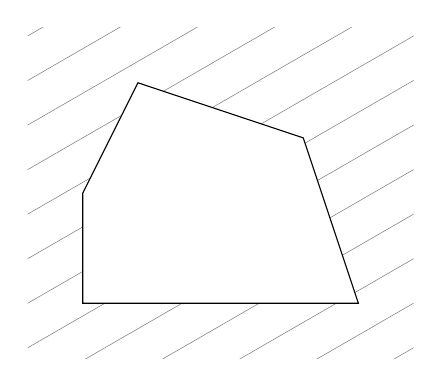
\begin{tikzpicture}[scale=0.7]%{{{
\clip  (-1,-1) rectangle (6,5);
%
% Hachures
\foreach \y in {-10,-9.3,...,11} \draw [gray, very thin, rotate=30] (-4,\y) to (18,\y);
%
% Ensemble sûr
\path [fill=white]
                 (0, 0) -- ++(0, 2)
            -- ++(1, 2) -- ++(3,-1)
            -- ++(1,-3) --    cycle;
%
% Ensemble sûr (redraw)
\draw            (0, 0) -- ++(0, 2)
            -- ++(1, 2) -- ++(3,-1)
            -- ++(1,-3) --    cycle;
%
\end{tikzpicture}%}}}
}
\hspace{5mm}
\subbottom[
  …mais pas celui des états atteints.
]{
\label{fig:ia-f2}
% 2
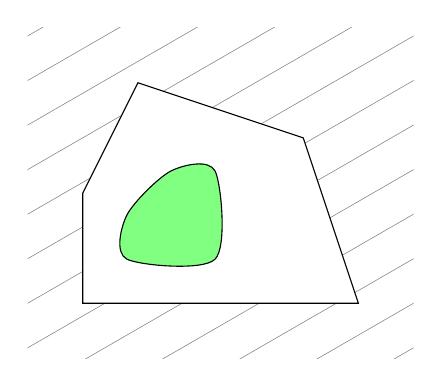
\begin{tikzpicture}[scale=0.7]%{{{
\clip  (-1,-1) rectangle (6,5);
%
% Hachures
\foreach \y in {-10,-9.3,...,11} \draw [gray, very thin, rotate=30] (-4,\y) to (18,\y);
%
% Ensemble sûr
\path [fill=white]
                 (0, 0) -- ++(0, 2)
            -- ++(1, 2) -- ++(3,-1)
            -- ++(1,-3) --    cycle;
%
% Ensemble sûr (redraw)
\draw            (0, 0) -- ++(0, 2)
            -- ++(1, 2) -- ++(3,-1)
            -- ++(1,-3) --    cycle;
%
% Comportement réel (sans erreurs)
\draw [fill=green!50,scale=0.8] plot[smooth cycle]
      coordinates{(1,1) (1,2) (2,3) (3,3) (3,1)};
%
\end{tikzpicture}%}}}
}

\subbottom[
  On construit donc une surapproximation calculable de la sémantique. Si
  celle-ci n'a pas d'erreur, on est assuré que le programme n'en aura pas non
  plus.
]{
\label{fig:ia-f3}
% 4
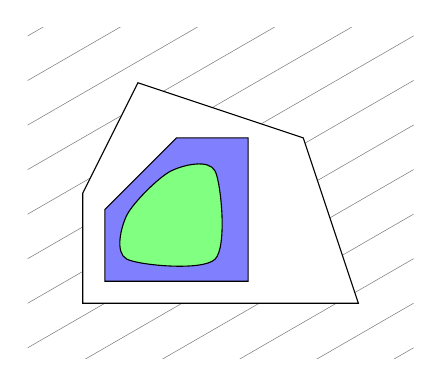
\begin{tikzpicture}[scale=0.7]%{{{
\clip  (-1,-1) rectangle (6,5);
%
% Hachures
\foreach \y in {-10,-9.3,...,11} \draw [gray, very thin, rotate=30] (-4,\y) to (18,\y);
%
% Ensemble sûr
\path [fill=white]
                 (0, 0) -- ++(0, 2)
            -- ++(1, 2) -- ++(3,-1)
            -- ++(1,-3) --    cycle;
%
% Ensemble sûr (redraw)
\draw            (0, 0) -- ++(0, 2)
            -- ++(1, 2) -- ++(3,-1)
            -- ++(1,-3) --    cycle;
%
% Approximation (précise)
\draw [fill=blue!50,scale around={1.3:(3,3)}]
           (1,1) -- (1,2)
        -- (2,3) -- (3,3)
        -- (3,1) -- cycle;
%
% Comportement réel (sans erreurs)
\draw [fill=green!50,scale=0.8] plot[smooth cycle]
      coordinates{(1,1) (1,2) (2,3) (3,3) (3,1)};
%
\end{tikzpicture}%}}}
}
\hspace{5mm}
\subbottom[
  Si on détecte une intersection, il n'est pas possible de savoir si elle est
  due à une erreur atteignable ou à une approximation trop laxe.
]{
\label{fig:ia-f4}
% 6
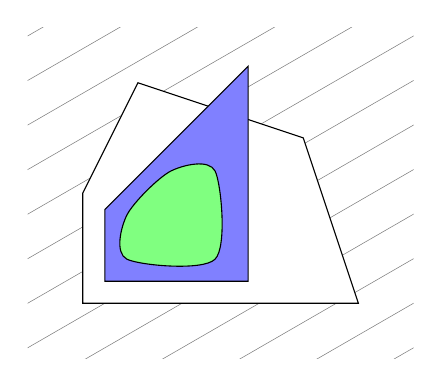
\begin{tikzpicture}[scale=0.7]%{{{
\clip  (-1,-1) rectangle (6,5);
%
% Hachures
\foreach \y in {-10,-9.3,...,11} \draw [gray, very thin, rotate=30] (-4,\y) to (18,\y);
%
% Ensemble sûr
\path [fill=white]
                 (0, 0) -- ++(0, 2)
            -- ++(1, 2) -- ++(3,-1)
            -- ++(1,-3) --    cycle;
%
% Ensemble sûr (redraw)
\draw            (0, 0) -- ++(0, 2)
            -- ++(1, 2) -- ++(3,-1)
            -- ++(1,-3) --    cycle;
%
% Approximation (imprécise)
\draw [fill=blue!50,scale around={1.3:(3,3)}]
            (1,1) -- (1,2)
         -- (3,4)
         -- (3,1) -- cycle;
%
% Comportement réel (sans erreurs)
\draw [fill=green!50,scale=0.8] plot[smooth cycle]
      coordinates{(1,1) (1,2) (2,3) (3,3) (3,1)};
%
\end{tikzpicture}%}}}
}

\caption{
  Surapproximation en interprétation abstraite.
  Il n'est pas possible de déterminer si l'ensemble des états atteignables
  est inclus dans l'ensemble des états sûrs (figure~\ref{fig:ia-f2}). En
  revanche, en construisant une surapproximation on peut parfois conclure
  (figures~\ref{fig:ia-f3} et~\ref{fig:ia-f4}).
}
\label{fig:ia}

\end{figure}%}}}

Les domaines les plus simples ne capturent aucune relation entre variables. Ce
sont des domaines non relationnels. On peut en citer quelques uns.

\paragraph{Le domaine des signes} capture uniquement le signe des variables
(figure~\ref{fig:dom-sig}).

\begin{figure}%{{{
\centering
\begin{tikzpicture}
\node at (1, 2) (t) {$\top$};
\node at (0, 1) (p) {$+$};
\node at (2, 1) (m) {$-$};
\node at (1, 0) (b) {$\bot$};
\draw (t) -- (p) -- (b);
\draw (t) -- (m) -- (b);
\end{tikzpicture}

\begin{align*}
\gamma~(+) = & \mathbb{R}^+ \\
\gamma~(-) = & \mathbb{R}^-
\end{align*}

\caption{Domaine des signes}
\label{fig:dom-sig}
\end{figure}%}}}

\paragraph{Le domaine des intervalles} retient les bornes de variations
extremales des variables (figure~\ref{fig:dom-intvl}).

\begin{figure} % {{{
\centering
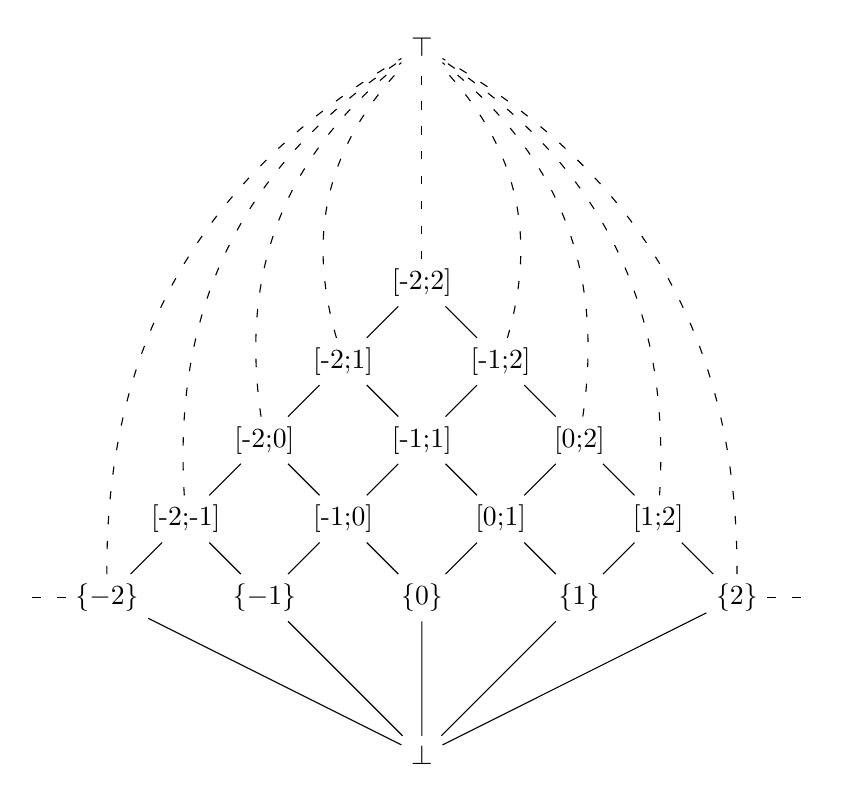
\begin{tikzpicture}
\node at (0,0)   (b)  {$\bot$};

\node at (-4,2) (cm2)   {$\{-2\}$};
\node at (-2,2) (cm1)   {$\{-1\}$};
\node at  (0,2)  (c0)   {$\{0\}$};
\node at  (2,2)  (c1)   {$\{1\}$};
\node at  (4,2)  (c2)   {$\{2\}$};

\node at (-3,3) (rm2m1) {[-2;-1]};
\node at (-1,3) (rm10)  {[-1;0]};
\node at  (1,3) (r01)   {[0;1]};
\node at  (3,3) (r12)   {[1;2]};

\node at (-2,4) (rm20)  {[-2;0]};
\node at  (0,4) (rm11)  {[-1;1]};
\node at  (2,4) (r02)   {[0;2]};

\node at (-1,5) (rm21)  {[-2;1]};
\node at  (1,5) (rm12)  {[-1;2]};

\node at  (0,6) (rm22)  {[-2;2]};

\node at  (0,9) (t)  {$\top$};

\draw (b) -- (cm2) -- (rm2m1) -- (rm20) -- (rm21) -- (rm22);
\draw (b) -- (cm1) -- (rm10) -- (rm11) -- (rm12);
\draw (b) -- (c0) -- (r01) -- (r02);
\draw (b) -- (c1) -- (r12);
\draw (b) -- (c2);

\draw (c2) -- (r12) -- (r02) -- (rm12) -- (rm22);
\draw (c1) -- (r01) -- (rm11) -- (rm21);
\draw (c0) -- (rm10) -- (rm20);
\draw (cm1) -- (rm2m1);

\draw[loosely dashed] (cm2)   to [bend left=30] (t);
\draw[loosely dashed] (rm2m1) to [bend left=30] (t);
\draw[loosely dashed] (rm20)  to [bend left=30] (t);
\draw[loosely dashed] (rm21)  to [bend left=30] (t);

\draw[loosely dashed] (rm22)  to (t);

\draw[loosely dashed] (rm12)   to [bend right=30] (t);
\draw[loosely dashed] (r02)   to [bend right=30] (t);
\draw[loosely dashed] (r12)   to [bend right=30] (t);
\draw[loosely dashed] (c2)    to [bend right=30] (t);

\draw[loosely dashed] (cm2) -- +(-1,0);
\draw[loosely dashed] (c2)  -- +(1,0);

\end{tikzpicture}

\caption{Domaine des intervalles}
\label{fig:dom-intvl}
\end{figure} % }}}

Lorsque plusieurs variables sont analysées en même temps, utiliser de tels
domaines revient à considérer un produit cartésien d'ensembles
(figure~\ref{fig:dom-cartesien})

Cela revient à oublier les relations entre les variables. Des domaines abstraits
plus précis permettent de retenir celles-ci. Pour ce faire, il faut modéliser
l'ensemble des valeurs des variables comme un tout. Parmi les domaines
relationnels courants on peut citer :

\begin{itemize}

\item Le domaine des polyèdres, historiquement l'un des premiers
domaines relationnels. Il permet de retenir tous les invariants affines entre
fonctions (figure~\ref{fig:dom-poly}).

\item Le domaine des zones permet de représenter des relations affines de
forme $v_i - v_j \le c$ (figure~\ref{fig:dom-zones}).

\item Le domaine des octogones est un compromis entre les polyèdres et les
zones. Il permet de représenter les relations $\pm v_i \pm v_j \le c$
(figure~\ref{fig:dom-octo}).

\end{itemize}

\begin{figure}%{{{

  \centering

  \subbottom[Un domaine non relationnel représente des produits cartésiens de%{{{
    domaines abstraits (ici, des intervalles).
  ]{
    \label{fig:dom-cartesien}
      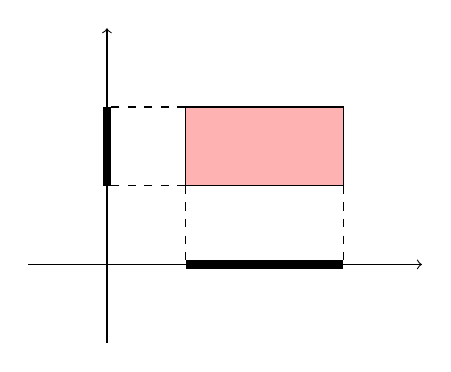
\begin{tikzpicture}
      \draw[->] (0,-1) -- (0,3);
      \draw[->] (-1,0) -- (4,0);
%
      \draw[fill=red!30] (1,1) rectangle (3,2);
%
      \draw[dashed] (3,1) -- (3,0);
      \draw[dashed] (1,1) -- (1,0);
%
      \draw[dashed] (1,2) -- (0,2);
      \draw[dashed] (1,1) -- (0,1);
%
      \draw[line width=3pt] (0,1) -- (0,2);
      \draw[line width=3pt] (3,0) -- (1,0);
%
      \end{tikzpicture}
  }%}}}
  \subbottom[Domaine des polyèdres]{%{{{
    \label{fig:dom-poly}
%
    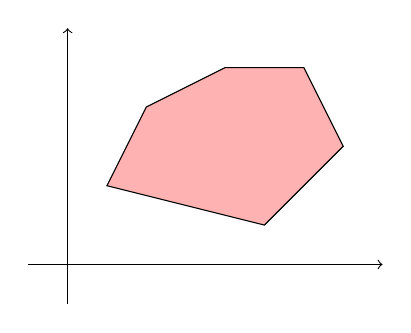
\begin{tikzpicture}[scale=0.5]
    \draw[->] (0,-1) -- (0,6);
    \draw[->] (-1,0) -- (8,0);
%
    \draw[fill=red!30] (1,2) -- (2,4) -- (4,5) -- (6,5) -- (7,3) -- (5,1) -- cycle;
%
    \end{tikzpicture}
  }%}}}

  \subbottom[Domaine des zones]{%{{{
    \label{fig:dom-zones}
%
    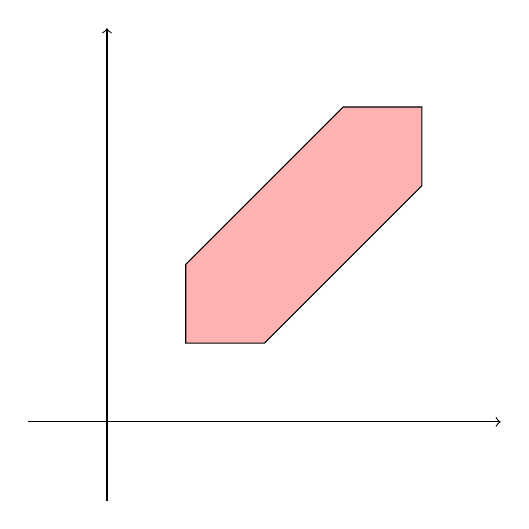
\begin{tikzpicture}
    \draw[->] (0,-1) -- (0,5);
    \draw[->] (-1,0) -- (5,0);
%
    \draw[fill=red!30] (1,2) -- (3,4) -- (4,4) -- (4,3) -- (2,1) -- (1,1) -- cycle;
%
    \end{tikzpicture}
  }%}}}
  \subbottom[Domaine des octaèdres]{%{{{
    \label{fig:dom-octo}
%
    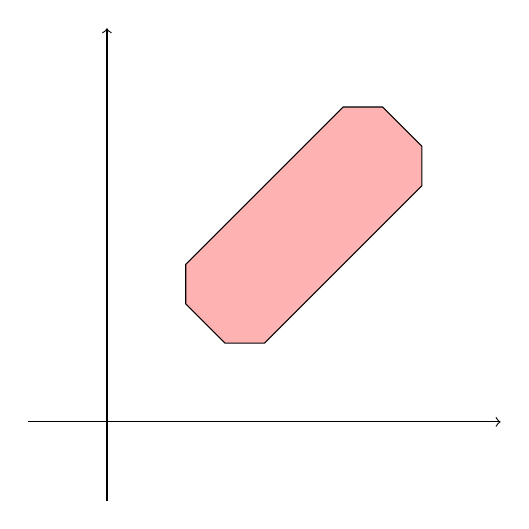
\begin{tikzpicture}
    \draw[->] (0,-1) -- (0,5);
    \draw[->] (-1,0) -- (5,0);
%
    \draw[fill=red!30] (1,1.5) -- (1,2) -- (3,4) -- (3.5,4) -- (4,3.5) -- (4,3) -- (2,1) -- (1.5,1) -- cycle;
%
    \end{tikzpicture}
  }%}}}

  \caption{Quelques domaines abstraits}
  \label{fig:dom-abstraits}
\end{figure}%}}}

En plus des domaines numériques, il est nécessaire d'employer des domaines
spécialisés dans la modélisation de la mémoire. Cela est nécessaire pour pouvoir
"suivre" les pointeurs. Par exemple, on peut représenter un pointeur par un
ensemble de variables possiblement pointées et une valeur abstraite représentant
le décalage (\emph{offset}) du pointeur par rapport au début de la zone mémoire.
Cette valeur peut elle-même être abstraite par un domaine numérique.

Au delà des domaines eux-mêmes, l'analyse se fait sous forme d'un calcul de
point fixe. La manière la plus simple est d'utiliser un algorithme de
\emph{liste de travail}, décrit par exemple dans~\cite{tapsoft95}. Les
raffinement en revanche sont nombreux.

Dès~\cite{Cousot77} il est remarqué que la terminaison de l'analyse n'est
assurée que si le treillis des valeurs abstraites est de hauteur finie, ou qu'un
opérateur d'élargissement (\emph{widening}) $\nabla$ est employé. L'idée est
qu'une fois qu'on a calculé quelques termes d'une suite croissante, on peut
réaliser une projection de celle ci. Par exemple, dans le domaine des
intervalles, $[0;2]~\nabla~[0;3] = [0;+\infty[$. On atteint alors un point fixe
mais qui est plus grand que celui qu'on aurait obtenu sans cette accélération :
on perd en précision. Pour en gagner, on peut redescendre sur le treillis des
points fixe avec une suite d'itérations décroissantes \cite{granger}. Dans
l'itération de point fixe, il est possible d'obtenir les résultats de manière
plus efficace en choisissant un ordre particulier dans les calculs des
sous-itérations\cite{policy}.

% TODO pas clair

En termes d'ingéniérie logicielle, implanter un analyseur statique est un défi
en soi. En plus des domaines abstraits, d'un itérateur, il faut traduire le code
source à analyser dans un langage, et traduire les résultats de l'analyse en un
ensemble d'"alarmes" à présenter à l'utilisateur.

Pour des retours d'expérience, on peut se référer aux descriptions d'
Astrée\cite{Astree04,Astree05,AstreeScale},
CGS \cite{cgs},
Coverity \cite{coverityBillion},
ou de Penjili (TODO)

% TODO pas top

Une interprétation abstraite est par construction sûre et incomplète, donc ce
qui sépare une bon analyseur d'un mauvais est sa précision. Dans le cas du
langage C, de nombreuses constructions rendent imprécises les analyses :

\begin{itemize}
\item les nombres flottants
(types \texttt{float}, \texttt{double} et \texttt{long double}) ont une
sémantique particulière, et il n'est pas correct d'"approcher" leur sémantique
par une sémantique dans $ℝ$. Afin d'être correct, il faut établir des domaines
spécifiques au flottant, comme~\cite{floatpoly}. Un tour d'horizon des
difficultés liées aux flottants est effectué dans~\cite{floatpitfalls}.

\item les pointeurs sur fonction
rendent floue la limite qui est habituellement présente entre instructions et
données. En leur présence il est impossible de faire une analyse de flot de
contrôle indépendante du flot de données. Pour pouvoir les traiter, il faut que
le domaine abstrait en question soit assez précis pour qu'un pointeur abstrait
se concrétise en un ensemble réduit de fonctions. Dans le cas où le domaine ne
peut pas borner l'ensemble des fonctions possibles et renvoie $\top$, l'analyse
ne peut pas continuer.

\item l'allocation dynamique
de données, présente dans le langage C par le biais des fonctions
\texttt{malloc} et \texttt{free}, modifie le modèle mémoire
nécessaire. Sans celle-ci, l'ensemble des zones mémoire possibles peut être
décrit statiquement : ce sont les noms de variable. Ce qu'introduit
\texttt{malloc} au langage, c'est une zone mémoire qui n'a pas de nom, et sur
laquelle on n'a qu'un pointeur.

% TODO, bof + expand

\item le transtypage (\emph{casts}) entre entiers et pointeurs
est particulièrement délicat à traiter. Dans les modèles abstraits, les
pointeurs sur données ou sur fonctions n'ont pas de représentation numérique,
seulement une représentation symbolique. Même dans l'exécution concrète, la
représentation numérique d'un pointeur est lié à de nombreux choix faits par
l'environnement d'exécution (comme la randomisation de l'espace d'adressage) qui
ne peuvent pas facilement être modélisés.

\end{itemize}

\subsection*{TODO}

\begin{itemize}
\item difficultés :

\begin{itemize}
\item
  récursion
\end{itemize}

\item produit réduit
\item CIL, autres front end
\item polyspace?
\item APRON?
\end{itemize}

\section{Typage}

La plupart des langages de programmation incorporent la notion de type, qui
permet de détecter ou d'empêcher de manipuler des données incompatibles entre
elles.

Nous avons vu dans le chapitre~\ref{cha:os} qu'au niveau du langage machine, les
seules données qu'un ordinateur manipule sont des nombres. Selon les opérations
effectuées, ils seront interprétés comme des entiers, des adresses mémoires, ou
des caractères. Pourtant il est clair que certaines opérations n'ont pas de
sens: par exemple, ajouter deux adresses, ou déréférencer le résultat d'une
division sont des comportements qu'on voudrait pouvoir empêcher.

En un mot, le but du typage est de classifier les objets et de restreindre les
opérations possibles selon la classe d'un objet : ``ne pas ajouter des pommes et
des oranges''. Le modèle qui permet cette classification est appelé
\emph{système de types} et est en général constitué d'un ensemble de
\emph{règles de typage}, comme ``un entier plus un entier égale un entier''.

Il y a deux grandes familles de systèmes de types, selon quand se fait la
vérification de types. On peut en effet l'effectuer au moment de l'exécution, ou
au contraire prévenir les erreurs à l'exécution en la faisant au moment de la
compilation (ou avant l'interprétation).

\paragraph{Typage dynamique :} dans ce cas, chaque valeur manipulée par le
programme est décorée d'une étiquette définissant comment interpréter la valeur
en question. Les règles de typage sont alors réalisées à l'exécution. Par
exemple, l'opérateur "$+$" vérifie que ces deux opérandes ont une étiquette
"entier", et construit alors une valeur obtenue en faisant l'addition des deux
valeurs, avec une étiquette "entier". Symboliquement :

\begin{verbatim}
fonction addition(x, y) {
  if ( (etiquette_type(x) != type_entier)
    || (etiquette_type(y) != type_entier)
    ) {
      erreur ("L'addition est seulement définie pour deux entiers")
  } else {
    vx = valeur(x)
    vy = valeur(y)
    v = addition_machine(vx, vy)
    return Valeur(valeur=v, type=type_entier)
  }
}
\end{verbatim}

Le langage Python~\link{python} utilise cette stratégie, qui est illustrée dans
la session interactive de la figure~\ref{fig:typage-dynamique}.

\begin{figure}
  \insertcode{typage-dynamique.pycon}
  \caption{Session Python présentant le typage dynamique}
  \label{fig:typage-dynamique}
\end{figure}

\paragraph{Typage statique :} dans ce cas on fait les vérifications à la
compilation. En quelque sorte, l'approche dynamique est pessimiste, puisqu'elle
demande de traiter très souvent le cas où les types ne sont pas corrects.
Intuitivement, dans le cas où toutes les fonctions se comportent bien, faire la
vérification est inutile. Pour vérifier ceci, on donne à chaque fonction un
contrat comme "si deux entiers sont passés, le fonction renverra un entier sans
provoquer d'erreur". Cet ensemble de contrats peut être vérifié statiquement par
le compilateur, à l'aide d'un système de types statique.

Ainsi la fonction "$+$" est typée \texttt{(int * int)} $→$ \texttt{int}. Les
règles permettant de vérifier le typage sont par exemple les suivantes :

\begin{itemize}
\item
  une constante entière est toujours de type \texttt{int}.
\item
  si $f$ a pour type $(t_1, …, t_n) → t$, que $e_1$ a pour type $t_1$,
  \ldots{}, que $e_n$ a pour type $t_n$, alors $f(e_1, …, e_n)$ a pour
  type $t_n$
\item
  si en considérant que $e_1$ a pour type $t_n$, …, et que $e_n$ a pour type
  $t_n$, on arrive à typer le corps de $f$ et que sa valeur de retour a alors
  pour type $t$,
  alors $f$ a pour type $(t_1, …, t_n) → t$
\end{itemize}

Cet ensemble de règles, une fois formalisé et implanté, est en général assez
efficace pour vérifier la correction d'un programme.

\paragraph{Typage fort ou faible :}

Si un système de types statique permet d'éliminer totalement la nécessité de
réaliser des tests de typage, on dit qu'il est \emph{fort}. Mais ce n'est que
rarement le cas. En effet, il peut y avoir des constructions au sein du langage
qui permettent de contourner le système de types, comme un opérateur de
transtypage\ref{fig:javacast}. À l'exécution, une erreur de types est levée :

\begin{figure}
  \insertcode{cast.java}
  \caption{Transtypage en Java}
  \label{fig:javacast}
\end{figure}

\begin{Verbatim}
Exception in thread "main" java.lang.ClassCastException:
    java.lang.Integer cannot be cast to java.lang.Float
        at Cast.main(Cast.java:5)
\end{Verbatim}

\paragraph{Polymorphisme :} parfois, il est trop restrictif de donner un unique
contrat à une fonction. Quel doit être le type d'une fonction ajoutant un
élément à une liste ?

En première approximation, on peut imaginer fournir une version du code par type
de données à manipuler. C'est la solution retenue par les premières versions du
langage Pascal, ce qui rendait très difficile l'écriture de
bibliothèques\cite{PascalNoEscape}.

Une amélioration peut être de générer à la compilation une fonction qui aurait
le même code mais des annotations de typage différentes : on obtient alors
plusieurs copies de la fonction qui sont chacunes spécialisées pour un type en
particulier. C'est la solution retenue par le langage C++.

En fait, si à l'exécution toutes les données sont représentées de manière
uniforme, il n'est pas nécessaire de créer plusieurs copies de la fonction.

\begin{figure}
  \insertcode{listappend.ml}
  \caption{Fonction de concaténation de listes en OCaml.}
  \label{fig:listappend}
\end{figure}

Par exemple, la fonction de la figure~\ref{fig:listappend} n'opère que sur la
structure du type liste (en utilisant ses constructeurs \texttt{{[}{]}} et
\listcons ainsi que le filtrage) : les éléments de \texttt{lx} et \texttt{ly} ne
sont pas manipulés à part pour les transférer dans le résultat.

Elle peut donc être typée avec n'importe quelle type 
$a~\textrm{list} → a~\textrm{list} → a~\textrm{list}$. Pour introduire cette
généricité, on modifie le système de types pour transformer :

\[ ∀ a. \textrm{append} :
   a~\textrm{list} → a~\textrm{list} → a~\textrm{list}
\]

en :

\[ \textrm{append} : ∀ a.
   a~\textrm{list} → a~\textrm{list} → a~\textrm{list}
\]

Au lieu d'associer à chaque expression un type, dans certains cas on lui associe
un schéma de types, instanciable en un type concret. Cette technique a été
décrite en premier dans~\cite{Milner78}.

\subsection*{TODO}

\begin{itemize}
\item
  incorporer la subsection d'après
\end{itemize}

\begin{center}\rule{3in}{0.4pt}\end{center}

L'approche par typage, plus légère, est séduisante. Pour les différents enjeux
des systèmes de types statiques, on pourra se référer à~\cite{TAPL}. Il est
possible d'encoder ce genre de propriétés dans un sytème de types, cf.
\cite{lightweight-static-capabilities} et \cite{LZ06a}.

\section{Qualificateurs de types}

Dans le cas particulier des vulnérabilités liées à une mauvaise utilisation de
la mémoire, les développeurs du noyau Linux ont ajouté un système d'annotations
au code source. Un pointeur peut être décoré d'une annotation
\texttt{\_\_kernel} ou \texttt{\_\_user} selon s'il est sûr ou pas. Celle-ci
sont ignorées par le compilateur, mais un outil d'analyse statique ad-hoc nommé
Sparse \link{sparse} peut être utilisé pour détecter les cas les plus simples
d'erreurs.

Ce système d'annotations sur les types a été formalisé sous le nom de
\emph{qualificateurs de types} : chaque type peut être décoré d'un ensemble de
qualificateurs (à la manière de \texttt{const}), et des règles de typage
permettent d'établir des propriétés sur le programme. Ces analyses ont été
implantée dans l'outil CQual
\cite{pldi99,usenix01,pldi02,cquk-usenix04,toplas-quals}. \todo{lister les
applications}.

\section{Logique de Hoare}

Une technique pour vérifier statiquement des propriétés sur la sémantique d'un
programme a été formalisée par Robert Floyd\cite{FloydMeaning} et Tony
Hoare\cite{hoare}.

Elle consiste à écrire les invariants qui sont maintenus à un point donné du
programme. Ces propositions sont écrites dans une logique $\mathcal{L}$.

Chaque instruction (ou \emph{commande}) $c$ est annotée d'une pré-condition $P$
et d'une post-condition $Q$, ce que l'on note $\hoare{P}{c}{Q}$. Cela signifie
que si $P$ est vérifiée et que l'exécution de $c$ se termine
\footnote{
  Comme dans la plupart des cas, la vérification de la terminaison d'un
  algorithme est réalisée de manière séparée.
  % TODO faire un chapeau général façon Devie?
  % 1/ Terminaison
  % 2/ Correction
  % 3/ Complexité
}
, alors $Q$ sera vérifiée.

En plus des règles de $\mathcal{L}$, des règles d'inférence traduisent la
sémantique du programme ; par exemple la règle de composition est :

\begin{mathpar}
  \irule{Hoare-Seq}
    { \hoare{P}{c_1}{Q} \\
      \hoare{Q}{c_2}{R}
    }{
      \hoare{P}{c_1;c_2}{R}
    }
\end{mathpar}

Les pré-conditions peuvent être renforcées et les post-conditions relaxées :

\begin{mathpar}
  \irule{Hoare-Consequence}
    { ⊢_{\mathcal{L}} P  ⇒ P' \\
      \hoare{P}{c}{Q} \\
      ⊢_{\mathcal{L}} Q' ⇒ Q
    }
    { \hoare{P'}{c}{Q'} }
\end{mathpar}

Il est alors possible d'annoter le programme avec ses invariants formalisés de
manière explicite dans $\mathcal{L}$. Ceux-ci seront vérifiés à la compilation.
% TODO à la compil?

La règle de conséquence permet de découpler les propriétés du programme lui-même
: plusieurs niveaux d'annotations sont possibles, du moins précis au plus
précis. En fait, il est même possible d'annoter chaque point de contrôle par
l'ensemble d'annotations vide : \hoare{T}{c}{T} est toujours vrai.

Augmenter graduellement les pré- et post-conditions est néanmoins assez
difficile, puisqu'il peut être nécessaire de modifier l'ensemble des conditions
à la fois.

Cette difficulté est mentionnée dans \cite{cssv}, où un système de programmation
par contrats est utilisé pour vérifier la correction de routines de manipulation
de chaînes en C.

Le système Spec\#, présenté dans \cite{krml136}, permet d'utiliser un système de
contrats sur le langage C\#.

\subsection*{TODO}

\begin{itemize}
\item
  citer JML (39, 40 dans \cite{krml136})
\item
  quand est-ce que le compile time suffit ? et le runtime nécessaire ?
\end{itemize}

\section{Assistants de preuves et systèmes de types dépendants}

\begin{itemize}
\item Dependent types
\item proof $:$ theorem $::$ type $:$ term
\item Coq
\item Agda, termination checker
\item proof irrelevance
\item Theorems for Free\cite{theoremsforfree}
\end{itemize}

% TODO

\section{Analyse dynamique}

Du côté de l'analyse dynamique, \cite{oakland10}\todo{et Perl ?}.

\section{Analyse de flot}

Ce que nous voulons vérifier peut être vue comme une propriété de flot. Un tour
d'horizon des problèmes et techniques existantes peut être trouvé
dans~\cite{sm-jsac03}.

\section{Divers}

Divers : Taint sequences \cite{mdv10},

Frama-C ?

CCurred ?
